\section{Задание №6 (Вариант 2)} \label{06-lab}

\subsection{Условие} \label{06-lab-condition}

Найти решение задачи целочисленного линейного программирования
симплекс- и геометрическим методами.

\begin{align*}
     & F = x_1 + x_2 \to \max \\
     & \begin{cases}
           x_1 + 2x_2 \leq 14   \\
           -5x_1 + 3x_2 \leq 15 \\
           2x_1 - 3x_2 \leq 12
       \end{cases}   \\
     & x_1, x_2 \in \N_0
\end{align*}

\subsection{Решение} \label{06-lab-solution}

\subsubsection{Симплекс-метод} \label{06-lab-solution-simplex}

\textbf{Решение общей задачи}

\begin{align*}
     & F = x_1 + x_2 \to \max \\
     & \begin{cases}
           x_1 + 2x_2 \leq 14   \\
           -5x_1 + 3x_2 \leq 15 \\
           2x_1 - 3x_2 \leq 12  \\
           x_1 \geq 0           \\
           x_2 \geq 0
       \end{cases}   \\
\end{align*}

Приведём ограничения к каноническому виду:

\[
    \begin{cases}
        F - x_1 - x_2 = 0       \\
        x_1 + 2x_2 + x_3 = 14   \\
        -5x_1 + 3x_2 + x_4 = 15 \\
        2x_1 - 3x_2 + x_5 = 12  \\
    \end{cases}
\]

Составим симплекс-таблицу:

\begin{table}[H]
    \centering
    \begin{tabular}{|c|c|c|c|c|c|c|c|c|}
        \hline
          & Базис & $x_1$ & $x_2$ & $x_3$ & $x_4$ & $x_5$ & $b_i$ & $\dfrac{b_i}{\text{решающий столбец}}$ \\ \hline
        ~ & $x_3$ & 1     & 2     & 1     & 0     & 0     & 14    & ~                                      \\ \hline
        ~ & $x_4$ & -5    & 3     & 0     & 1     & 0     & 15    & ~                                      \\ \hline
        ~ & $x_5$ & 2     & -3    & 0     & 0     & 1     & 12    & ~                                      \\ \hline
        ~ & F     & -1    & -1    & 0     & 0     & 0     & 0     & ~                                      \\ \hline
    \end{tabular}
\end{table}

\begin{table}[H]
    \centering
    \begin{tabular}{|c|c|>{\columncolor{mycolumncolor}}c|c|c|c|c|c|c|}
        \hline
                  & Базис & $x_1$             & $x_2$ & $x_3$ & $x_4$ & $x_5$ & $b_i$ & $\dfrac{b_i}{\text{решающий столбец}}$ \\ \hline
        $\cdot 2$ & $x_3$ & 1                 & 2     & 1     & 0     & 0     & 14    & 14                                     \\ \hline
        $\cdot 2$ & $x_4$ & -5                & 3     & 0     & 1     & 0     & 15    & -3 < 0                                 \\ \hline
        \myrowcolor
        ~         & $x_5$ & \mycellcolor 2    & -3    & 0     & 0     & 1     & 12    & 6 \leftarrow min                       \\ \hline
        $\cdot 2$ & F     & -1 \leftarrow min & -1    & 0     & 0     & 0     & 0     & ~                                      \\ \hline
    \end{tabular}
\end{table}

\begin{table}[H]
    \centering
    \begin{tabular}{|c|c|>{\columncolor{mycolumncolor}}c|c|c|c|c|c|c|}
        \hline
          & Базис & $x_1$             & $x_2$ & $x_3$ & $x_4$ & $x_5$ & $b_i$ & $\dfrac{b_i}{\text{решающий столбец}}$ \\ \hline
        ~ & $x_3$ & 2                 & 4     & 2     & 0     & 0     & 28    & 14                                     \\ \hline
        ~ & $x_4$ & -10               & 6     & 0     & 2     & 0     & 30    & -3 < 0                                 \\ \hline
        \myrowcolor
        ~ & $x_5$ & \mycellcolor 2    & -3    & 0     & 0     & 1     & 12    & 6 \leftarrow min                       \\ \hline
        ~ & 2F    & -2 \leftarrow min & -2    & 0     & 0     & 0     & 0     & ~                                      \\ \hline
    \end{tabular}
\end{table}

\begin{table}[H]
    \centering
    \begin{tabular}{|c|c|c|>{\columncolor{mycolumncolor}}c|c|c|c|c|c|}
        \hline
          & Базис & $x_1$ & $x_2$             & $x_3$ & $x_4$ & $x_5$ & $b_i$ & $\dfrac{b_i}{\text{решающий столбец}}$ \\ \hline
        ~ & $x_3$ & 0     & 7                 & 2     & 0     & -1    & 16    &                                        \\ \hline
        ~ & $x_4$ & 0     & -9                & 0     & 2     & 5     & 90    &                                        \\ \hline
        ~ & $x_1$ & 2     & -3                & 0     & 0     & 1     & 12    &                                        \\ \hline
        ~ & 2F    & 0     & -5 \leftarrow min & 0     & 0     & 1     & 12    & ~                                      \\ \hline
    \end{tabular}
\end{table}

\begin{table}[H]
    \centering
    \begin{tabular}{|c|c|c|>{\columncolor{mycolumncolor}}c|c|c|c|c|c|}
        \hline
                  & Базис & $x_1$ & $x_2$             & $x_3$ & $x_4$ & $x_5$ & $b_i$ & $\frac{b_i}{\text{решающий столбец}}$ \\ \hline
        \myrowcolor
        ~         & $x_3$ & 0     & \mycellcolor7     & 2     & 0     & -1    & 16    & $\frac{16}{7}$                        \\ \hline
        $\cdot 7$ & $x_4$ & 0     & -9                & 0     & 2     & 5     & 90    & -10 < 0                               \\ \hline
        $\cdot 7$ & $x_1$ & 2     & -3                & 0     & 0     & 1     & 12    & -4 < 0                                \\ \hline
        $\cdot 7$ & 2F    & 0     & -5 \leftarrow min & 0     & 0     & 1     & 12    & ~                                     \\ \hline
    \end{tabular}
\end{table}

\begin{table}[H]
    \centering
    \begin{tabular}{|c|c|c|>{\columncolor{mycolumncolor}}c|c|c|c|c|c|}
        \hline
          & Базис & $x_1$ & $x_2$              & $x_3$ & $x_4$ & $x_5$ & $b_i$ & $\dfrac{b_i}{\text{решающий столбец}}$ \\ \hline
        \myrowcolor
        ~ & $x_3$ & 0     & \mycellcolor 7     & 2     & 0     & -1    & 16    & $\frac{16}{7}$                         \\ \hline
          & $x_4$ & 0     & -63                & 0     & 14    & 35    & 630   & -10 < 0                                \\ \hline
          & $x_1$ & 14    & -21                & 0     & 0     & 7     & 84    & -4 < 0                                 \\ \hline
          & 14F   & 0     & -35 \leftarrow min & 0     & 0     & 7     & 84    & ~                                      \\ \hline
    \end{tabular}
\end{table}

\begin{table}[H]
    \centering
    \begin{tabular}{|c|c|c|c|c|c|c|c|c|}
        \hline
          & Базис           & $x_1$          & $x_2$         & $x_3$ & $x_4$          & $x_5$ & $b_i$           & $\dfrac{b_i}{\text{решающий столбец}}$ \\ \hline
        ~ & $x_2$           & 0              & \mycellcolor7 & 2     & 0              & -1    & \mycellcolor16  &                                        \\ \hline
          & $x_4$           & 0              & 0             & 18    & \mycellcolor14 & 26    & \mycellcolor774 &                                        \\ \hline
          & $x_1$           & \mycellcolor14 & 0             & 6     & 0              & 4     & \mycellcolor132 &                                        \\ \hline
          & \mycellcolor14F & 0              & 0             & 10    & 0              & 2     & \mycellcolor164 & Все > 0                                \\ \hline
    \end{tabular}
\end{table}

Получили $x^* = (\dfrac{66}{7}, \dfrac{16}{7}),\ f^* = \dfrac{82}{7}$.

\textbf{Решение целочисленной задачи}

Как видим, в оптимальном решении присутствуют дробные значения. Для отсечения Гомори нам нужно знать дробные части оптимальных переменных:

$q_1 = {x^*_1} = \dfrac{66}{7} - 9 = \dfrac{3}{7}$;
$q_2 = {x^*_2} = \dfrac{16}{7} - 2 = \dfrac{2}{7}$

Большая дробная часть у переменной $x_1$, поэтому будем использовать её для отсечения Гомори.

Для начала нормализуем последнюю симплекс-таблицу:

\begin{table}[H]
    \centering
    \begin{tabular}{|c|c|c|c|c|c|c|c|}
        \hline
          & Базис & $x_1$ & $x_2$ & $x_3$            & $x_4$ & $x_5$              & $b_i$                \\ \hline
        ~ & $x_2$ & 0     & 1     & $ \frac{ 2}{ 7}$ & 0     & $- \frac{ 1}{ 7}$  & $ \frac{ 16}{ 7}$    \\ \hline
          & $x_4$ & 0     & 0     & $ \frac{ 9}{ 7}$ & 1     & $ \frac{ 13}{ 7} $ & $  \frac{387 }{ 7} $ \\ \hline
          & $x_1$ & 1     & 0     & $ \frac{ 3}{ 7}$ & 0     & $ \frac{2}{7} $    & $\frac{66}{7}$       \\ \hline
          & F     & 0     & 0     & $ \frac{ 5}{ 7}$ & 0     & $ \frac{ 1}{ 7}$   & $ \frac{82}{7} $     \\ \hline
    \end{tabular}
\end{table}

Смотрим в строку $x_1$ и составляем отсечение Гомори: $q_1 - \sum\limits_{j=1}^n q_{1j}x_j \leq 0$

Найдём $q_{1j}$: $q_{11} = 0, q_{12} = 0, q_{13} = \dfrac{3}{7}, q_{14} = 0, q_{15} = \dfrac{ 2}{ 7}$.

Отсечение Гомори: $ \frac{ 3}{ 7} - \frac{ 3}{ 7}x_3 - \frac{ 2}{ 7}x_5 \leq 0 $

Получили новое ограничение. Переписываем ограничение в каноническом виде и добавляем его в симплекс-таблицу: $ \frac{ 3}{ 7}x_3 + \frac{ 2}{ 7}x_5 - x_6 = \frac{ 3}{ 7} $

\begin{table}[H]
    \centering
    \begin{tabular}{|c|c|c|c|c|c|c|c|c|c|}
        \hline
          & Базис & $x_1$ & $x_2$ & $x_3$            & $x_4$ & $x_5$              & $x_6$ & $b_i$                \\ \hline
        ~ & $x_2$ & 0     & 1     & $ \frac{ 2}{ 7}$ & 0     & $- \frac{ 1}{ 7}$  & 0     & $ \frac{ 16}{ 7}$    \\ \hline
          & $x_4$ & 0     & 0     & $ \frac{ 9}{ 7}$ & 1     & $ \frac{ 13}{ 7} $ & 0     & $  \frac{387 }{ 7} $ \\ \hline
          & $x_1$ & 1     & 0     & $ \frac{ 3}{ 7}$ & 0     & $ \frac{2}{7} $    & 0     & $\frac{66}{7}$       \\ \hline
        ~ & $x_6$ & 0     & 0     & $\frac{ 3}{ 7}$  & 0     & $ \frac{ 2}{ 7} $  & -1    & $\frac{3}{7}$        \\ \hline
          & F     & 0     & 0     & $ \frac{ 5}{ 7}$ & 0     & $ \frac{ 1}{ 7}$   & 0     & $ \frac{82}{7} $     \\ \hline
    \end{tabular}
\end{table}

Теперь видим, что нужно немного уменьшить $F$, чтобы получить целочисленные решения. Проще всего это сделать, увеличивая $x_5$, то есть $x_5$ --- разрешающий столбец.

\begin{table}[H]
    \centering
    \begin{tabular}{|c|c|c|c|c|c|>{\columncolor{mycolumncolor}}c|c|c|c|}
        \hline
                          & Базис & $x_1$ & $x_2$ & $x_3$            & $x_4$ & $x_5$                          & $x_6$ & $b_i$                & $\dfrac{b_i}{\text{решающий столбец}}$ \\ \hline
        $\cdot 7 \cdot 2$ & $x_2$ & 0     & 1     & $ \frac{ 2}{ 7}$ & 0     & $- \frac{ 1}{ 7}$              & 0     & $ \frac{ 16}{ 7}$    & -16 < 0                                \\ \hline
        $\cdot 7 \cdot 2$ & $x_4$ & 0     & 0     & $ \frac{ 9}{ 7}$ & 1     & $ \frac{ 13}{ 7} $             & 0     & $  \frac{387 }{ 7} $ & $ \frac{ 387}{ 7}$                     \\ \hline
        $\cdot 7$         & $x_1$ & 1     & 0     & $ \frac{ 3}{ 7}$ & 0     & $ \frac{2}{7} $                & 0     & $\frac{66}{7}$       & 33                                     \\ \hline
        \myrowcolor
        $\cdot 7$ ~       & $x_6$ & 0     & 0     & $\frac{ 3}{ 7}$  & 0     & $ \mycellcolor \frac{ 2}{ 7} $ & -1    & $\frac{3}{7}$        & $ \frac{ 3}{ 2}$ \leftarrow min        \\ \hline
        $\cdot 7 \cdot 2$ & F     & 0     & 0     & $ \frac{ 5}{ 7}$ & 0     & $ \frac{ 1}{ 7}$               & 0     & $ \frac{82}{7} $     &                                        \\ \hline
    \end{tabular}
\end{table}

\begin{table}[H]
    \centering
    \begin{tabular}{|c|c|c|c|c|c|>{\columncolor{mycolumncolor}}c|c|c|c|}
        \hline
         & Базис & $x_1$ & $x_2$ & $x_3$ & $x_4$ & $x_5$          & $x_6$ & $b_i$ & $\dfrac{b_i}{\text{решающий столбец}}$ \\ \hline
         & $x_2$ & 0     & 14    & 4     & 0     & -2             & 0     & 32    & -16 < 0                                \\ \hline
         & $x_4$ & 0     & 0     & 18    & 14    & 26             & 0     & 774   & 774                                    \\ \hline
         & $x_1$ & 7     & 0     & 3     & 0     & 2              & 0     & 66    & 33                                     \\ \hline
        \myrowcolor
         & $x_6$ & 0     & 0     & 3     & 0     & \mycellcolor 2 & -7    & 3     & $ \frac{ 3}{ 2}$ \leftarrow min        \\ \hline
         & 14F   & 0     & 0     & 10    & 0     & 2              & 0     & 164   &                                        \\ \hline
    \end{tabular}
\end{table}

\begin{table}[H]
    \centering
    \begin{tabular}{|c|c|c|c|c|c|c|c|c|}
        \hline
         & Базис & $x_1$ & $x_2$ & $x_3$ & $x_4$ & $x_5$ & $x_6$ & $b_i$ \\ \hline
         & $x_2$ & 0     & 14    & 7     & 0     & 0     & 7     & 35    \\ \hline
         & $x_4$ & 0     & 0     & -21   & 14    & 0     & 91    & 774   \\ \hline
         & $x_1$ & 7     & 0     & 0     & 0     & 0     & 7     & 63    \\ \hline
         & $x_5$ & 0     & 0     & 3     & 0     & 2     & -7    & 3     \\ \hline
         & 14F   & 0     & 0     & 7     & 0     & 0     & 7     & 161   \\ \hline
    \end{tabular}
\end{table}

Получили оптимальное решение $x^* = (9, \frac{ 5}{ 2})$, $x_1$ стало целочисленным, $x_2$ --- ещё нет. Повторим процедуру для $x_2$.

\begin{table}[H]
    \centering
    \begin{tabular}{|c|c|c|c|c|c|c|c|c|}
        \hline
         & Базис & $x_1$ & $x_2$ & $x_3$            & $x_4$ & $x_5$ & $x_6$            & $b_i$          \\ \hline
         & $x_2$ & 0     & 1     & $ \frac{ 1}{ 2}$ & 0     & 0     & $ \frac{ 1}{ 2}$ & $ \frac{5}{2}$ \\ \hline
    \end{tabular}
\end{table}

$q_2 = \frac{ 1}{ 2}$

$q_{21} = 0, q_{22} = 0, q_{23} = \frac{ 1}{ 2}, q_{24} = 0, q_{25} = 0, q_{26} = \frac{ 1}{ 2}$

Отсечение Гомори: $ \frac{ 1}{ 2} - \frac{ 1}{ 2}x_3 - \frac{ 1}{ 2}x_6 \leq 0 $. Приведём к каноническому виду: $ \frac{ 1}{ 2}x_3 + \frac{ 1}{ 2}x_6 - x_7 = \frac{ 1}{ 2} $ и добавим в симплекс-таблицу:

\begin{table}[H]
    \centering
    \begin{tabular}{|c|c|c|c|c|c|c|c|c|c|}
        \hline
         & Базис & $x_1$ & $x_2$ & $x_3$             & $x_4$ & $x_5$ & $x_6$             & $x_7$ & $b_i$             \\ \hline
         & $x_2$ & 0     & 1     & $ \frac{ 1}{ 2}$  & 0     & 0     & $ \frac{ 1}{ 2}$  & 0     & $ \frac{5}{2}$    \\ \hline
         & $x_4$ & 0     & 0     & $- \frac{ 3}{ 2}$ & 1     & 0     & $ \frac{ 13}{ 2}$ & 0     & $ \frac{337}{7}$  \\ \hline
         & $x_1$ & 1     & 0     & 0                 & 0     & 0     & 1                 & 0     & 9                 \\ \hline
         & $x_5$ & 0     & 0     & $ \frac{ 3}{ 2}$  & 0     & 1     & $- \frac{ 7}{ 2}$ & 0     & $ \frac{ 3}{ 2}$  \\ \hline
         & $x_7$ & 0     & 0     & $ \frac{ 1}{ 2}$  & 0     & 0     & $\frac{ 1}{ 2}$   & -1    & $ \frac{1}{2}$    \\ \hline
         & F     & 0     & 0     & $ \frac{1}{2}$    & 0     & 0     & $ \frac{1}{2}$    & 0     & $ \frac{ 23}{ 2}$ \\ \hline
    \end{tabular}
\end{table}

Теперь видим, что нужно немного уменьшить $F$, чтобы получить целочисленные решения. Проще всего это сделать, увеличивая $x_3$, то есть $x_3$ --- разрешающий столбец. Вводим его в базис вместо $x_7$:

\begin{table}[H]
    \centering
    \begin{tabular}{|c|c|c|c|>{\columncolor{mycolumncolor}}c|c|c|c|c|c|}
        \hline
         & Базис & $x_1$ & $x_2$ & $x_3$                        & $x_4$ & $x_5$ & $x_6$             & $x_7$ & $b_i$             \\ \hline
         & $x_2$ & 0     & 1     & $ \frac{ 1}{ 2}$             & 0     & 0     & $ \frac{ 1}{ 2}$  & 0     & $ \frac{5}{2}$    \\ \hline
         & $x_4$ & 0     & 0     & $- \frac{ 3}{ 2}$            & 1     & 0     & $ \frac{ 13}{ 2}$ & 0     & $ \frac{337}{7}$  \\ \hline
         & $x_1$ & 1     & 0     & 0                            & 0     & 0     & 1                 & 0     & 9                 \\ \hline
         & $x_5$ & 0     & 0     & $ \frac{ 3}{ 2}$             & 0     & 1     & $- \frac{ 7}{ 2}$ & 0     & $ \frac{ 3}{ 2}$  \\ \hline
        \myrowcolor
         & $x_7$ & 0     & 0     & \mycellcolor$ \frac{ 1}{ 2}$ & 0     & 0     & $\frac{ 1}{ 2}$   & -1    & $ \frac{1}{2}$    \\ \hline
         & F     & 0     & 0     & $ \frac{1}{2}$               & 0     & 0     & $ \frac{1}{2}$    & 0     & $ \frac{ 23}{ 2}$ \\ \hline
    \end{tabular}
\end{table}

\begin{table}[H]
    \centering
    \begin{tabular}{|c|c|c|c|>{\columncolor{mycolumncolor}}c|c|c|c|c|c|}
        \hline
         & Базис & $x_1$ & $x_2$ & $x_3$                        & $x_4$ & $x_5$ & $x_6$           & $x_7$ & $b_i$            \\ \hline
         & $x_2$ & 0     & 1     & 0                            & 0     & 0     & 0               & 0     & 2                \\ \hline
         & $x_4$ & 0     & 0     & 0                            & 1     & 0     & 8               & -3    & $ \frac{340}{7}$ \\ \hline
         & $x_1$ & 1     & 0     & 0                            & 0     & 0     & 1               & 0     & 9                \\ \hline
         & $x_5$ & 0     & 0     & 0                            & 0     & 1     & -5              & 0     & 0                \\ \hline
        \myrowcolor
         & $x_7$ & 0     & 0     & \mycellcolor$ \frac{ 1}{ 2}$ & 0     & 0     & $\frac{ 1}{ 2}$ & -1    & $ \frac{1}{2}$   \\ \hline
         & F     & 0     & 0     & 0                            & 0     & 0     & 0               & 1     & 11               \\ \hline
    \end{tabular}
\end{table}

Получили оптимальное целочисленное решение $x^* = (9, 2)$, если подставим в функцию, то получим $f^* = 11$.

\textbf{Ответ:} $x^* = (9, 2),\ f^* = 11$. \label{06-lab-answer-simplex}

\subsubsection{Геометрический метод} \label{06-lab-solution-geom}

\textbf{Решение общей задачи}

\begin{align*}
     & F = x_1 + x_2 \to \max \\
     & \begin{cases}
           x_1 + 2x_2 \leq 14   \\
           -5x_1 + 3x_2 \leq 15 \\
           2x_1 - 3x_2 \leq 12  \\
           x_1 \geq 0           \\
           x_2 \geq 0
       \end{cases}   \\
\end{align*}

Найдём вектор градиента функции $F(x_1, x_2)$:

\[
    \overrightarrow{grad}F(x_1, x_2) = \left\{\deriv{F}{x_1}(x_1, x_2), \deriv{F}{x_2}(x_1, x_2)\right\} = \left\{1, 1\right\}
\]

Приведём ограничения к более наглядному виду:

\[
    \begin{cases}
        x_2 \leq -\dfrac{1}{2}x_1 + 7 \\
        x_2 \leq \dfrac{5}{3}x_1 + 5  \\
        x_2 \geq \dfrac{2}{3}x_1 - 4  \\
        x_1 \geq 0                    \\
        x_2 \geq 0
    \end{cases}
\]

Используя библиотеку $matplotlib$ для $Python$, построим график(\href{https://github.com/retrobannerS/optimization_methods/blob/main/python/06-lab/01-graphic.py}{код для построения графика}):

\begin{figure}[H]
    \leftskip-1.5cm
    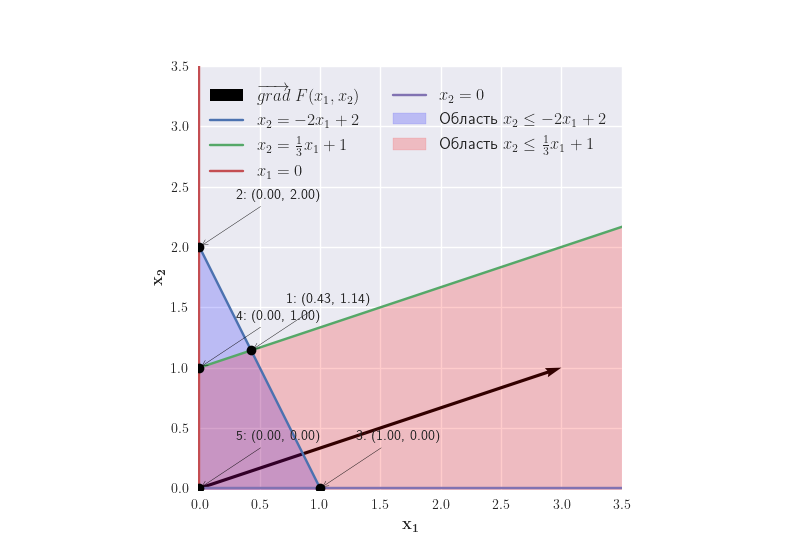
\includegraphics[width=1.2\textwidth]{images/06-lab/01-graphic.png}
    \caption{График общей задачи задания 6.}
    \label{06-lab-01-graphic}
\end{figure}

В условную область попадают все точки пересечения, кроме точек 3 и 4.
Подставим подходящие точки в функцию $F$ и выведем её значения в этих точках:

\begin{lstlisting}[language=text]
    Значение F в точке 1 равно 7.46
    Значение F в точке 2 равно 11.71
    Значение F в точке 5 равно 5.00
    Значение F в точке 6 равно 6.00
    Значение F в точке 7 равно 0.00
\end{lstlisting}

Таким образом оптимальное решение и максимизированная функция:
\[x^* = \left(\dfrac{66}{7}, \dfrac{16}{7}\right),\ f^* = \dfrac{82}{7}.\]

\textbf{Решение целочисленной задачи}

Из решения (\hyperref[06-lab-solution-simplex]{симплекс-методом}) мы знаем, что первое отсечение Гомори имеет вид:

$ \frac{ 3}{ 7} - \frac{ 3}{ 7}x_3 - \frac{ 2}{ 7}x_5 \leq 0 $.

$x_3$ и $x_5$ выражаются через $x_1$ и $x_2$ следующим образом:

$x_3 = 14 - x_1 - 2x_2$, $x_5 = 12 -2x_1 + 3x_2$.

Таким образом, новое ограничение:

$ \frac{ 3}{ 7} - \frac{ 3}{ 7}(14 - x_1 - 2x_2) - \frac{ 2}{ 7}(12 -2x_1 + 3x_2) = \frac{ 3}{ 7} - 6 + \frac{ 3}{ 7}x_1 + \frac{ 6}{ 7} x_2 - \frac{ 24}{ 7} + \frac{ 4}{ 7}x_1 - \frac{ 6}{ 7}x_2 = x_1 - 9 \leq 0 $.

То есть новое ограничение: $x_1 \leq 9$.

Строим график(\href{https://github.com/retrobannerS/optimization_methods/blob/main/python/06-lab/02-graphic.py}{код для построения графика}):

\begin{figure}[H]
    \leftskip-1.5cm
    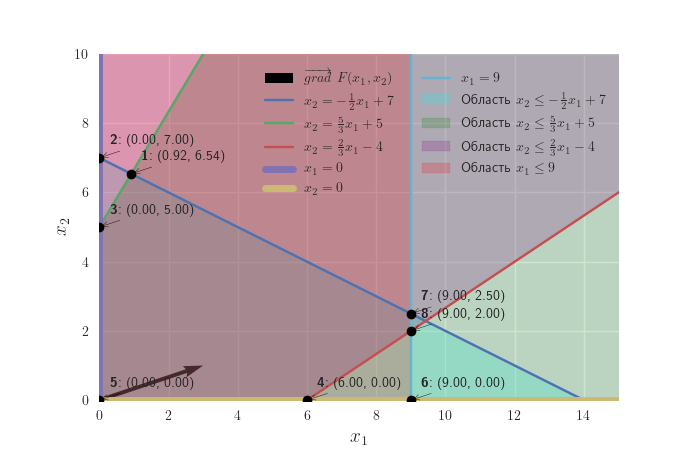
\includegraphics[width=1.2\textwidth]{images/06-lab/02-graphic.png}
    \caption{График №1 целочисленной задачи задания 6.}
    \label{06-lab-02-graphic}
\end{figure}

Нам подходят все точки, кроме 2 и 6. Подставим подходящие точки в функцию $F$ и выведем её значения в этих точках:

\begin{lstlisting}[language=text]
    Значение F в точке 1 равно 7.46
    Значение F в точке 3 равно 5.00
    Значение F в точке 4 равно 6.00
    Значение F в точке 5 равно 0.00
    Значение F в точке 7 равно 11.50
    Значение F в точке 8 равно 11.00
\end{lstlisting}

Таким образом оптимальное решение и максимизированная функция:
\[x^* = \left(9,\ \dfrac{5}{2}\right),\ f^* = \dfrac{23}{2}\]

Значения снова нецелочисленные. Возьмём второе отсечение Гомори из решения (\hyperref[06-lab-solution-simplex]{симплекс-методом}):

$ \frac{ 1}{ 2} - \frac{ 1}{ 2}x_3 - \frac{ 1}{ 2}x_6 \leq 0 $.

$x_3$ и $x_6$ выражаются через $x_1$ и $x_2$ следующим образом:

$x_3 = 14 - x_1 - 2x_2$, $x_6 = \frac{ 3}{ 7}x_3 + \frac{ 2}{ 7}x_5 - \frac{ 3}{ 7}$.

$x_5 = 12 -2x_1 + 3x_2 \Rightarrow x_6 = \frac{ 3}{ 7}(14 - x_1 - 2x_2) + \frac{ 2}{ 7}(12 -2x_1 + 3x_2) - \frac{ 3}{ 7} \Rightarrow x_6 = 9 - x_1$.

Таким образом, новое ограничение:

$ \frac{ 1}{ 2} - \frac{ 1}{ 2}(14 - x_1 - 2x_2) - \frac{ 1}{ 2}(9 - x_1) = \frac{ 1}{ 2} - 7 + \frac{ 1}{ 2}x_1 + x_2 - \frac{ 9}{ 2} + \frac{ 1}{ 2}x_1 = x_1 + x_2 - 11 \leq 0 $.

Или в упрощённом виде: $x_2 \leq -x_1 + 11$.

Добавим это ограничение на график(\href{https://github.com/retrobannerS/optimization_methods/blob/main/python/06-lab/03-graphic.py}{код для построения графика}):

\begin{figure}[H]
    \leftskip-1.5cm
    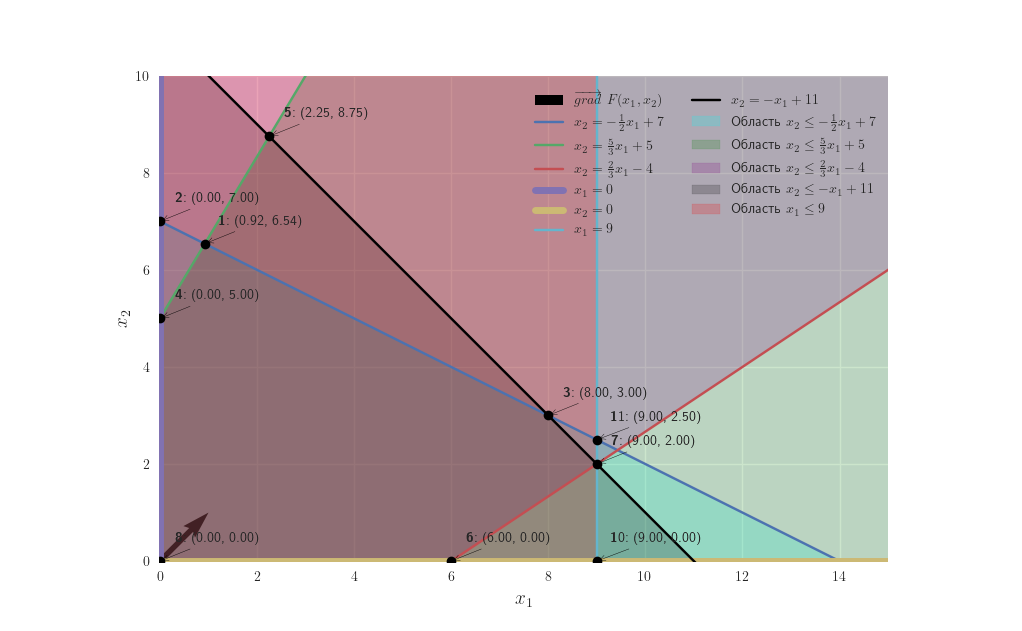
\includegraphics[width=1.2\textwidth]{images/06-lab/03-graphic.png}
    \caption{График №2 целочисленной задачи задания 6.}
    \label{06-lab-03-graphic}
\end{figure}

Подходят все точки с графика, кроме 2, 5, 10, 11. Подставим подходящие точки в функцию $F$ и выведем её значения в этих точках:

\begin{lstlisting}[language=text]
    Значение F в точке 1 равно 7.46
    Значение F в точке 3 равно 11.00
    Значение F в точке 4 равно 5.00
    Значение F в точке 6 равно 6.00
    Значение F в точке 7 равно 11.00
    Значение F в точке 8 равно 0.00
\end{lstlisting}

Таким образом у нас есть даже два оптимальных решения:
\[x^* = (9, 2),\ f^* = 11\]
\[\tilde{x^*} = (8, 3),\ f^* = 11\]

\textbf{Ответ:} $x^* = (9, 2),\ \tilde{x^*} = (8, 3),\ f^* = 11$.\label{06-lab-answer-geom}

\newpage